\documentclass[11pt,english]{article}
\usepackage[latin9]{inputenc}
\usepackage[letterpaper]{geometry}
\geometry{verbose,tmargin=1in,bmargin=1in,lmargin=1in,rmargin=1in}
\usepackage{babel}
\usepackage{amsmath}
\usepackage{amssymb}
\usepackage{capt-of}
\usepackage{graphicx}
\usepackage[usenames,dvipsnames]{color}
\usepackage{latexsym}
\usepackage{xspace}
\usepackage{pdflscape}
\usepackage[hyphens]{url}
\usepackage[colorlinks]{hyperref}
\usepackage{enumerate}
\usepackage{hyperref}
\usepackage{float}
\usepackage{array}
\usepackage{tikz}
\usetikzlibrary{shapes}
\usepackage{algorithm2e}
\setcounter{MaxMatrixCols}{20}

\newcommand{\rthree}{\mathbb{R}^3}
\title{CIS 580 Homework 1 \\
Due: Monday}
 \author{Gabrielle Merritt}
 
\date{}

\begin{document}
\maketitle
\section*{ Camera Model }
\subsection*{CCD of iPhone 6}
The iPhone uses a sony isx014 cmos sensor with a 4.6 mm diagonal. Most likely dimensions are close to 3.67 mm x  2.76 mm.
\linebreak source: \url{ http://www.sony.net/Products/SC-HP/cx_news_archives/img/pdf/vol_70/isx014.pdf}
\subsection*{Sensor Pixel Resolution}
Pixel resolution is approximately 8.08 Megapixels ~ 7.21 pixels per $micron^2$
and pixel size $ =1.12 micron square$ 
\subsection*{Focal Length}
iPhone focal length for the iPhone6 is 29 mm
\subsection*{Measurement} 
Since I have the distance between myself and building $d_1$ and I know the properties of my camera 
I can calculate the height by using the Camera Propeties matrix. 
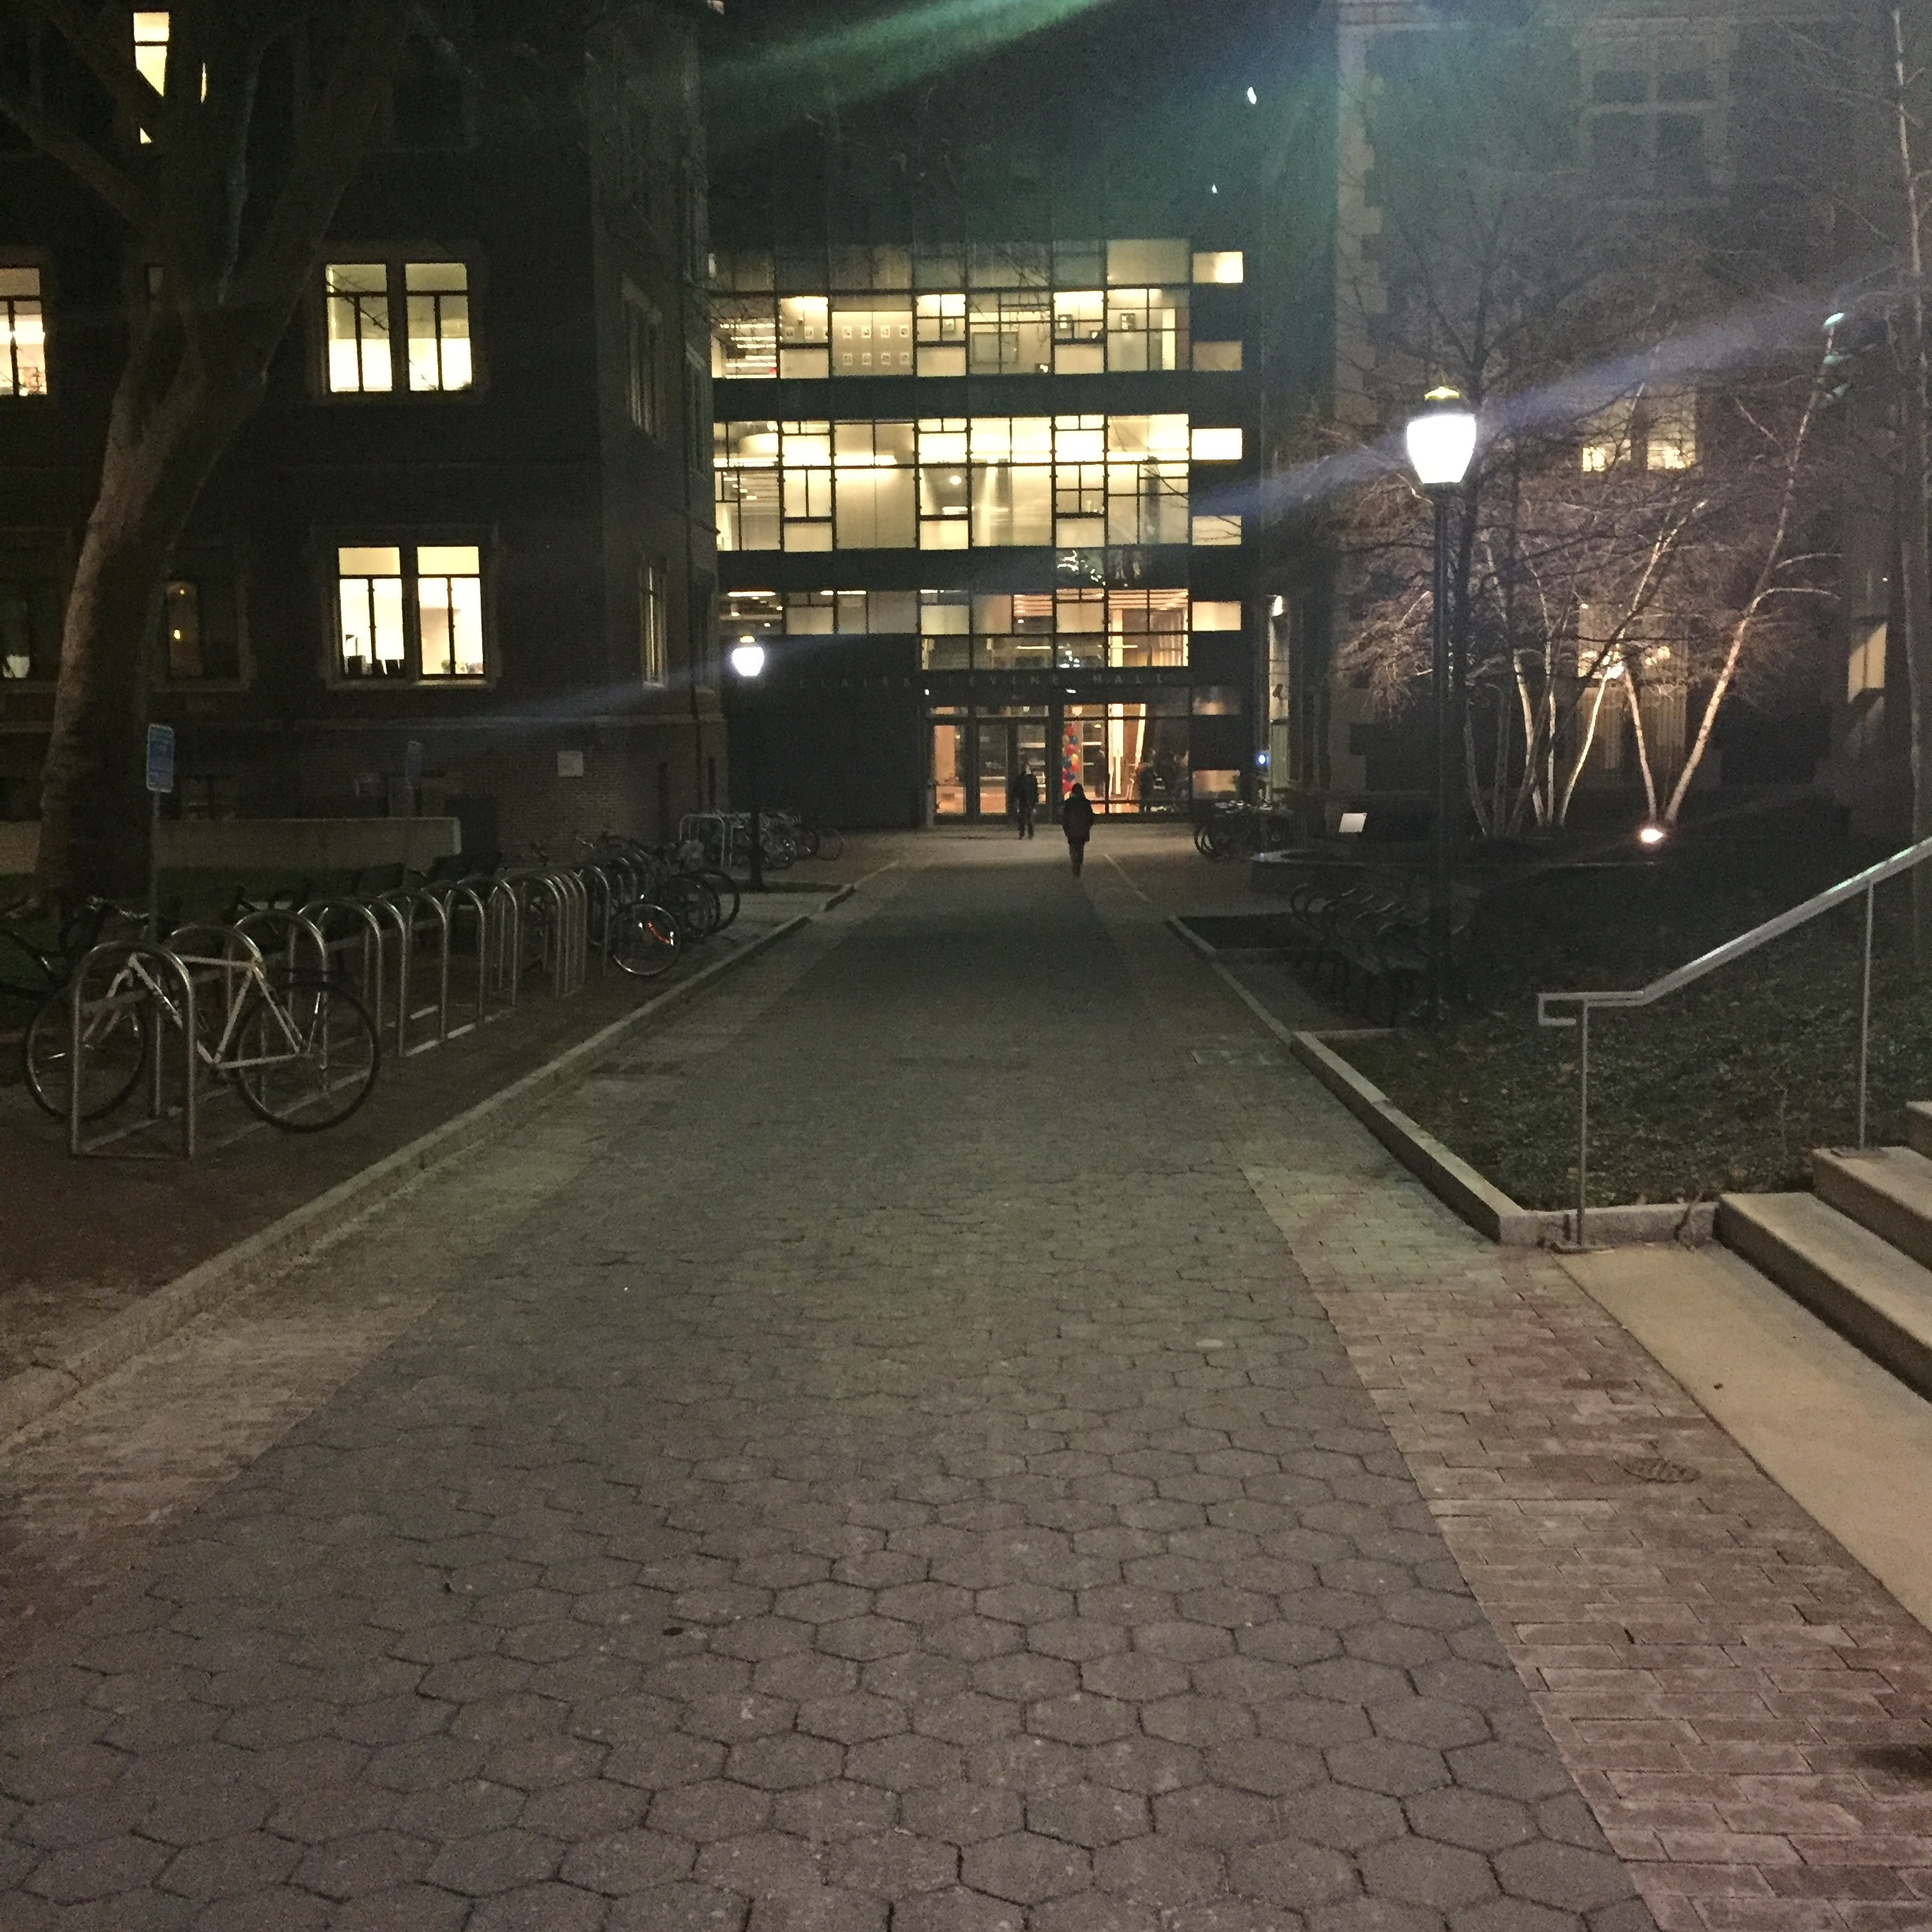
\includegraphics[width = \linewidth]{IMG_2529.jpg}
\begin{align*}
K^{-1} \begin{vmatrix}
\lambda u \\ \lambda v \\ \lambda 
\end{vmatrix} = \begin{pmatrix}
X \\ Y \\ Z 
\end{pmatrix}
\end{align*}
since we know Z (the distance from the camera to the building) we can simplify the calculation to 
we can solve for the world Y ( height) of the building. 
\begin{align*}
f = 29mm 
Z = 44805 mm 
\lambda = Z 
K = \begin{pmatrix}
f & 0 & 0 \\ 
0 & f & 0 \\ 
0 & 0 & 1 \\ 
\end{pmatrix} 
\text{So filling in the values we have}
K^{-1} \begin{pmatrix} \lambda 1566 \\ \lambda 15 \\ \lambda \end{pmatrix} = \begin{pmatrix} X \\ Y \\ Z \end{pmatrix} 
Y = 27810 mm 
\end{align*} 
The actual height of Levine is around 23 meters tall but since I was on a hill, I think this is a pretty close estimate 


\section*{Locate camera optical center by converging lines}
\subsection*{Camera Tilted Forward vs Camera Tilted Backwards}
If I Tilt the camera forwards it appears the lines converge at the horizon of the image. This is probably because since the camera is placed such that the radiating lines are parallel in the camera views, they appear to converge at infinity, which in this case is the edge of the image. 
\subsection*{Large Camera Optical Center}
Considering that the lines are diverging this means that the optical center is probably closer to point B, indictating that the focal length of the camera is much longer than the iphone camera. 

\section*{Estimating Height of Objects}
\subsection*{compute vanishing poitn on z axis} 
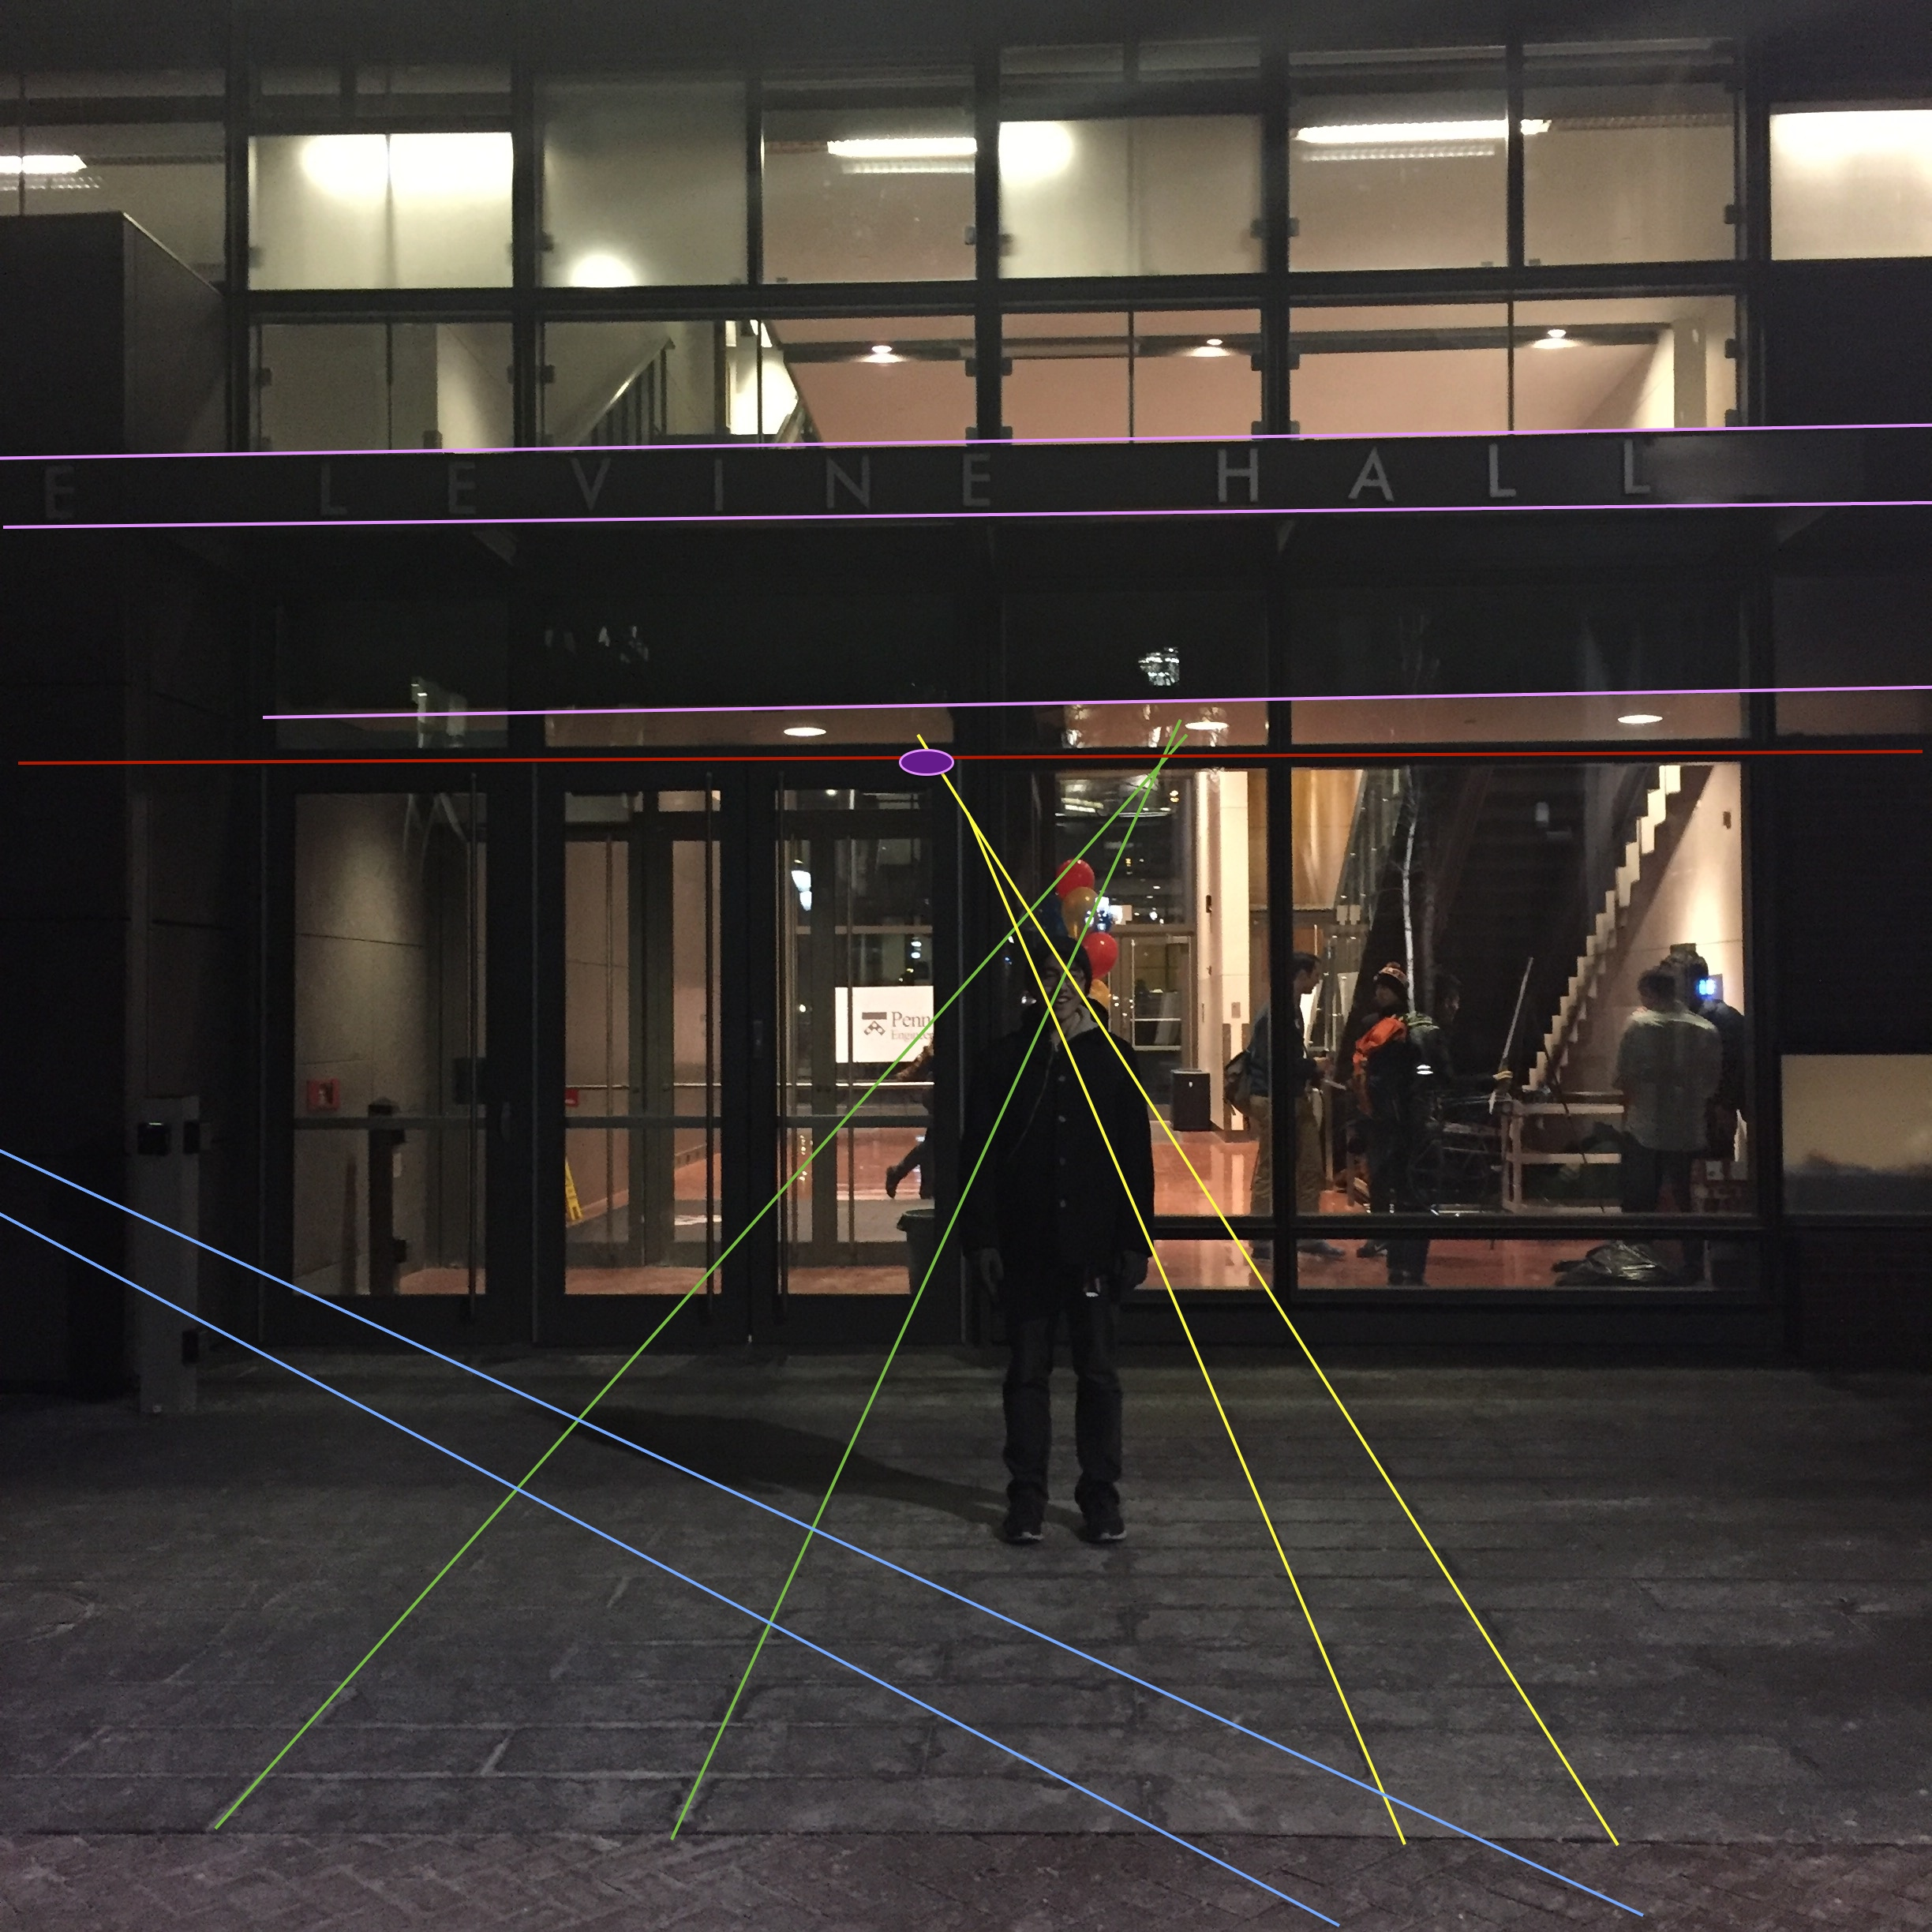
\includegraphics[width = \linewidth]{IMG_2525.jpg}
	vp =  -194676 pixels
\subsection*{compute height of levine door}
My friend is 1778 mm tall 
and 6267 mm from the camera 
\paragraph{}
By finding the conversion between the pixel at Rei's feet and pixel value at his height, 
and use that to find a conversion of pixels to distance for objects at Rei's distance.
then by finding angle betwee the top of Rei's head and the camera, we can find the height of the door at Rei's distance from the camera
and use the angle to find the actual distance between Rei and the door. tan(alpha) $/$ (distance between Rei's head and top of door)
now that we have the distance between my friend and the door we know the total distance to the door and can use similar triangles to find the total height of the door. \\ 
The levine door is about  
2404 mm high 

\section*{Dolly Zoom}
I think there is something very wrong with the renderer 
my K matrix is correct , but it only works if I flip the x and y of the pixel center, which is incorrect. 
I'm not sure how to fix this I've wasted about 2 days dealing with this so im just turning it in 
\paragraph{}
for project my equations are 

\begin{align}
K =\begin{pmatrix}f& 0 &p_y \\ 0 & f& p_x\\ 0& 0 &1\end{pmatrix} 
\begin{pmatrix} x \\ y \\ z\end{pmatrix} = K \begin{pmatrix} X \\ Y\\ Z\end{pmatrix}
\end{align}
\paragraph{}
for compute f 
since we are moving back at a set rate we simply want to have the new focal length keep object A in frame with side A1A2 keeping its original height of 400 pixels and 4 units
to get the conversion.
I've tried everything I sort of can't get this to work at all



\end{document}
